\subsection{Where}
\begin{center}

\textit{A che tipo di sito sono arrivato?}

\end{center}
\begin{flushleft}
Nella homepage del sito compare, in font sans serif di dimensione
più grande rispetto al resto del testo presente nella pagina e con un buon
contrasto rispetto al grigio di sfondo, il motto: \\
\quotes{Your complete web analytics toolkit} \\
Grazie a questa informazione l'utente sa di trovarsi in un sito che offre
strumenti di ricerca per il web. \\
    \begin{figure}[ht]
    \centering
    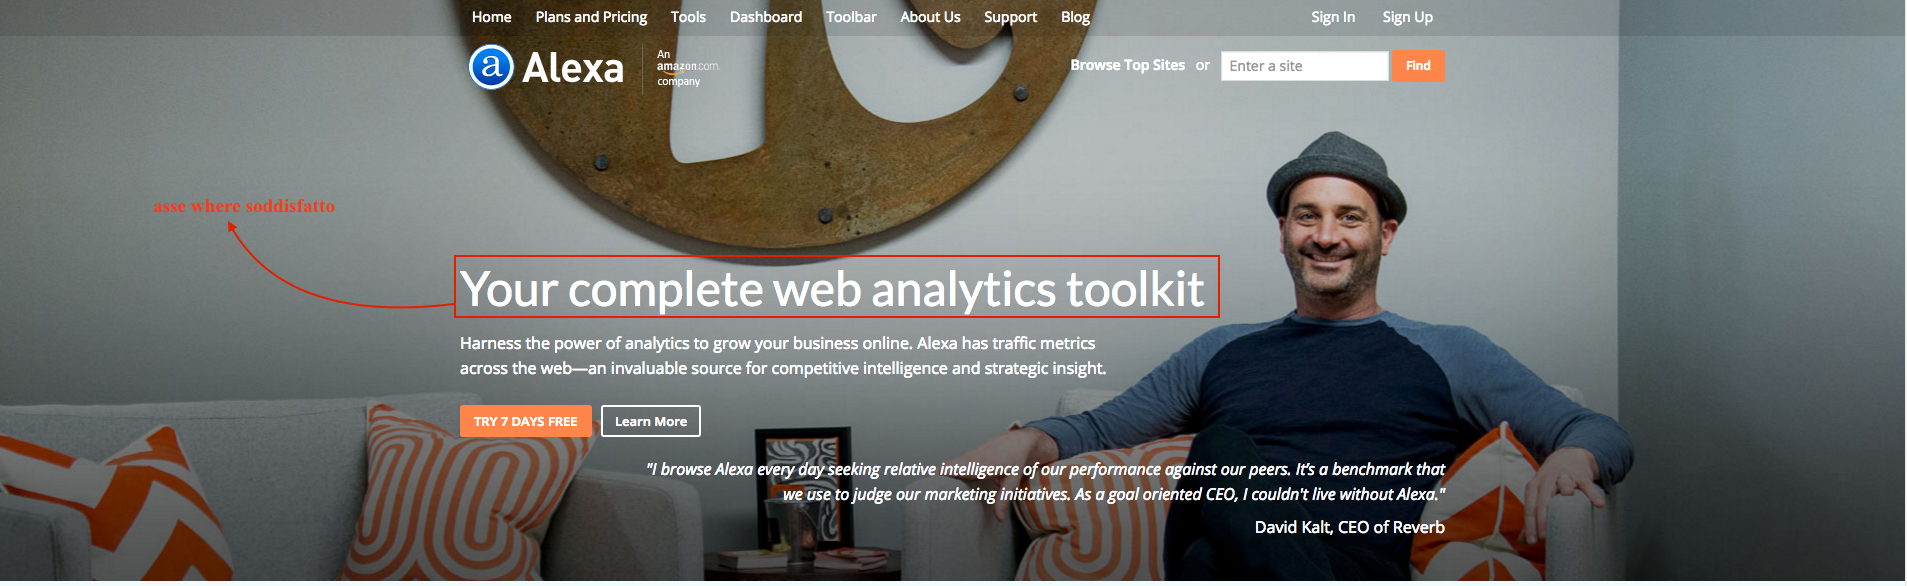
\includegraphics[scale=0.25,keepaspectratio]{{figure/3/where}.png}
    \caption{Homepage: in evidenza l'asse where}
    \end{figure}
    \FloatBarrier
Risultato : \textbf{8}
\end{flushleft}